%=================================================
% UNIDAD 5
%================================================

\chapter{Compacidad}

En esta unidad desarrollaremos el concepto de conjunto compacto y
otros relacionados. Los conjuntos compactos tienen la propiedad de
poder ser ``aproximados'' por conjuntos finitos, y por ello
heredan algunas propiedades de estos.

\section{Definici\'on de conjuntos compactos y precompactos}

Empezaremos por introducir lo que denominaremos conjuntos
\index{precompactos}.

\begin{definicion}  Diremos que un conjunto $A$ de un e.m. $(X,d)$ es precompacto
si para cada $\epsilon>0$ existe una cantidad finita de conjuntos
de di\'ametro menor que $\epsilon$ cuya uni\'on contiene a  $A$.
En otras palabras existen conjuntos $A_i$, $i=1,...,n$, con
$\delta(A_i)<\epsilon$ que satisfacen:
\[
    A\subset \bigcup\limits_{i=1}^nA_i.
\]
\end{definicion}

Veamos algunos ejemplos de conjuntos precompactos y de conjuntos
que no lo son.

\begin{ejemplo} Cualquier intervalo acotado de $\rr$ es
precompacto. Para justificar esta aseveraci\'on, tomemos
$\epsilon>0$ y un intervalo cualquiera de extremos $a$ y $b$.
Elijamos $n$ suficientemente grande para que $1/n<\epsilon$.
Entonces los conjuntos
\[
    I_k:=\bigl[\frac{k}{n},\frac{k+1}{n}\bigr]
\]
satisfacen la definici\'on.
\end{ejemplo}

\begin{ejemplo}\label{ejem,cubpre} Cualquier conjunto  acotado en el espacio euclideo
$\rr^n$ es precompacto. Sea $A\subset\rr^n$ un conjunto acotado.
Por ser $A$ acotado, est\'a contenido en un cubo de la forma
$C:=[-m,m]\times\dots\times [-m,m]=[-m,m]^n$. En virtud del
Ejercicio \vref{ejer,subpreespre} es suficiente demostrar que $C$
es precompacto. Sea $\epsilon>0$. Tomemos $k$ suficientemente
grande para que
\begin{equation}\label{eq,defk}
    \frac{2m}{\epsilon}<\sqrt{k}
\end{equation}
Ahora, partimos cada intervalo $[-m,m]$ en $k$ subintervalos de la
misma longitud $1/k$.

\begin{figure}[h]
\begin{center}
    \psfrag{a}{$\frac{2m}{k}$}
    \psfrag{b}{$\frac{2m}{\sqrt{k}}$}
    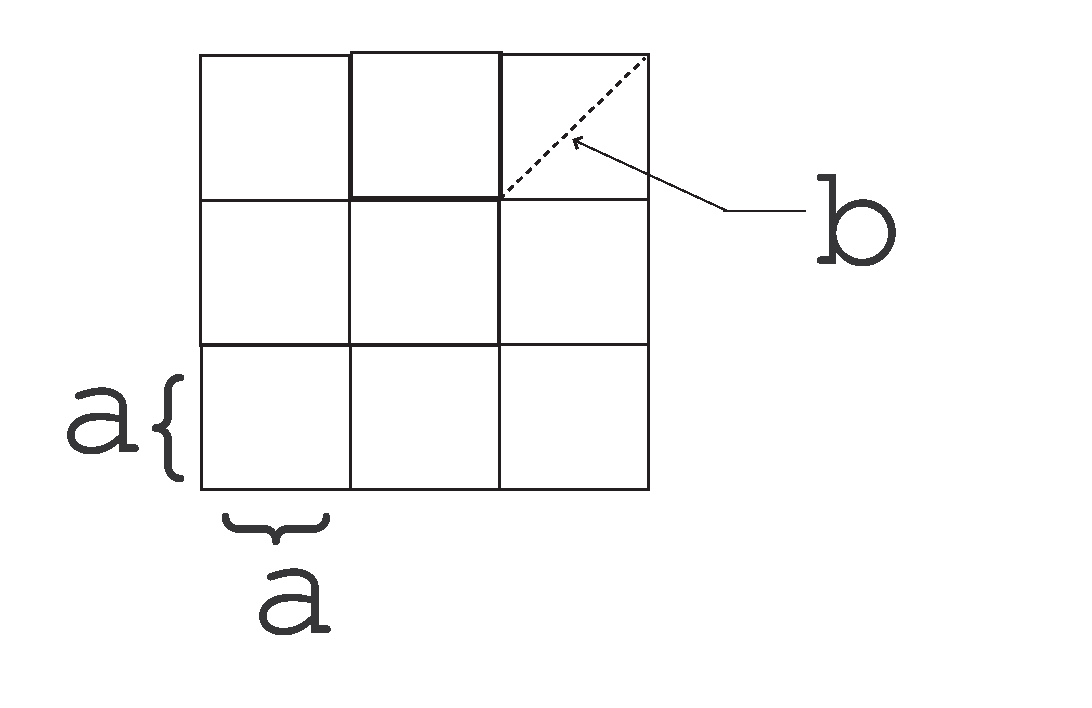
\includegraphics[height=6cm, width=10cm]{cubpre.eps}
    \caption{Construcci\'on del Ejemplo
    \ref{ejem,cubpre}}\label{fig,cubpre}
\end{center}
\end{figure}

Como puede observarse en la Figura \ref{fig,cubpre}, nos quedan
determinados $k^n$ cubos que cubren el cubo $C$. Cada uno de estos
cubos m\'as chicos tiene di\'ametro $2m/\sqrt{k}$, por
consiguiente, por la desigualdad \ref{eq,defk}, el di\'ametro de
ellos es menor que $\epsilon$.
\end{ejemplo}

No es cierto, en general, que todo conjunto acotado en un e.m. sea
precompacto. Los siguientes ejemplos muestran esto.

\begin{ejemplo} Sea $(X,d)$ un e.m. discreto con $X$ infinito. El
conjunto $X$ es acotado, de hecho $\delta(X)=1$; sin embargo no
podemos cubrir $X$ con conjuntos de di\'ametro menor que 1/2
(cualquier n\'umero menor que 1 servir\'{\i}a). Esto ocurre debido
a que si un conjunto en un e.m. discreto tiene m\'as de un
elemento entonces su di\'ametro es 1. As\'{\i}, si cubrimos $X$
con una cantidad finita de conjuntos, alguno de los conjuntos del
cubrimiento necesariamente tiene m\'as de un elemento, de lo
contrario $X$ ser\'{\i}a finito, por consiguiente el di\'ametro de
este conjunto es 1, por lo cual no puede ser menor que $1/2$.
\end{ejemplo}

\begin{ejemplo}\label{ejem,contnopre} En $C([0,1])$, con la m\'etrica del Ejemplo
\vref{ejem,distsobrecont}, la bola $\overline{B(0,1)}$ (0 denota
la funci\'on que es constantemente igual a 0) no es un conjunto
precompacto. Para ver esto definimos la siguiente funci\'on:

\[
    f(x):=\left\{%
\begin{array}{ll}
    4(x-\frac12), & \hbox{si $\frac12\leq x\leq \frac34$;} \\
    -4(x-1), & \hbox{si $\frac34\leq x\leq 1$;} \\
    0, & \hbox{para los restantes $x$;} \\
\end{array}
\right.
\]
y la siguiente sucesi\'on de funciones $f_n(x):=f(2^nx)$. En la
Figura \ref{fig,contnopre} puede verse las gr\'aficas de algunas
de las funciones de la sucesi\'on.

\begin{figure}[h]
\begin{center}
    \psfrag{f1}{$f_1$}
    \psfrag{f2}{$f_2$}
    \psfrag{f3}{$f_3$}
    \psfrag{f4}{$f_4$}
    \psfrag{1}{$1$}
    \psfrag{12}{$\frac12$}
    \psfrag{14}{$\frac14$}
    \psfrag{18}{$\frac18$}
    \psfrag{116}{$\frac{1}{16}$}
    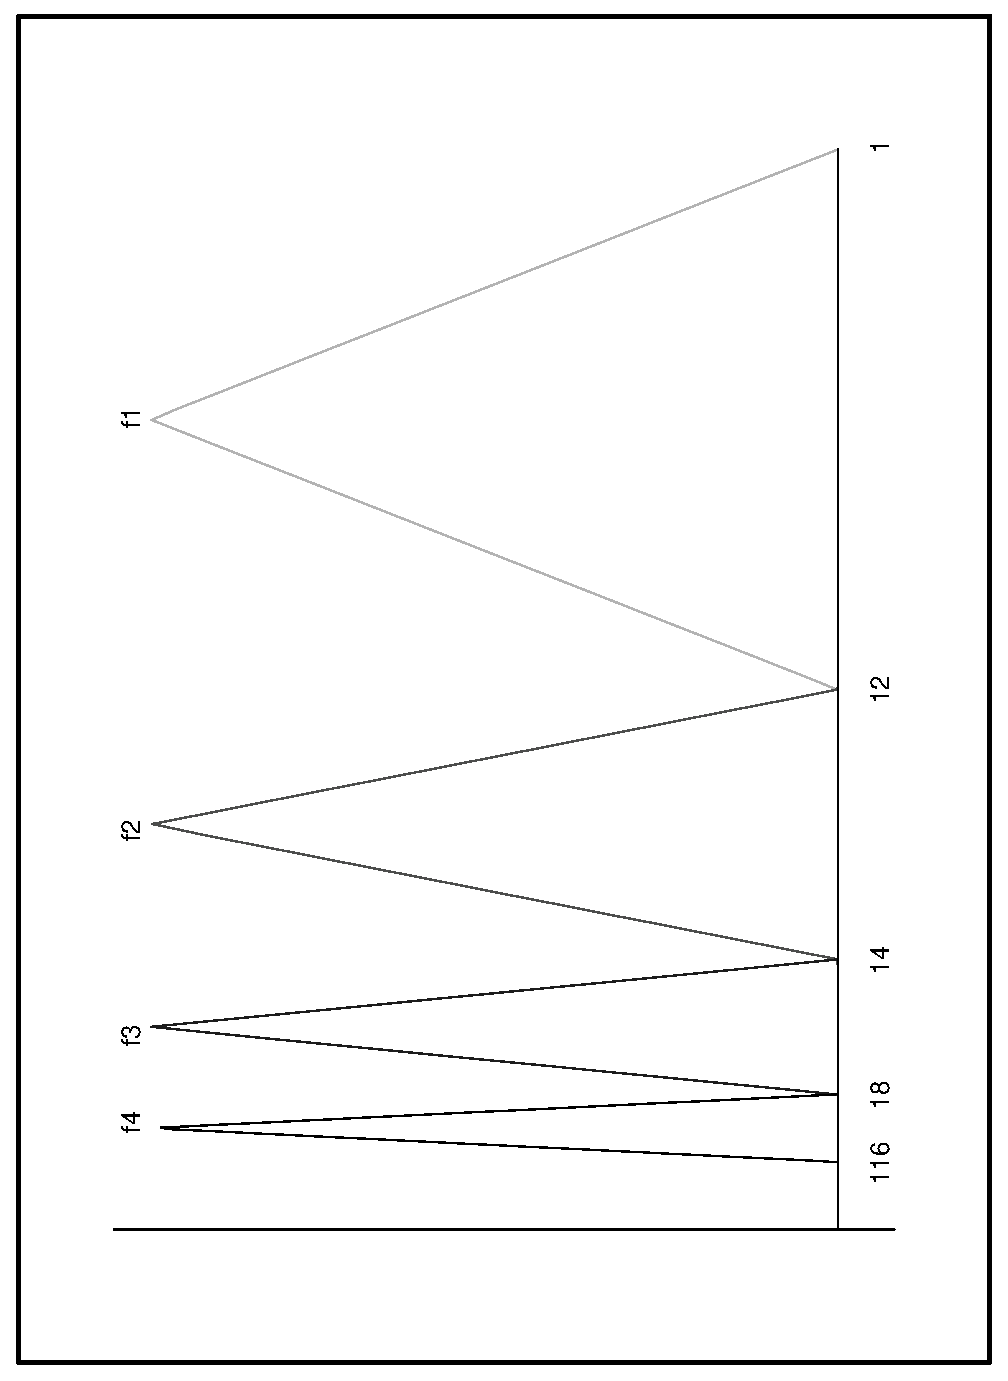
\includegraphics[height=12cm,
    width=7cm,angle=-90]{noprecom.eps}
    \caption{Funciones del Ejemplo
    \ref{ejem,contnopre}}\label{fig,contnopre}
\end{center}
\end{figure}

Puede demostrarse que la distancia de cualquiera de las funciones
de la sucesi\'on a otra es igual a 1. De modo que $f_n\in
\overline{B(0,1)}$. Sea $C:=\{f_n:n\in\nn\}$, observemos que como
subespacio $C$ resulta ser un e.m. discreto, as\'{\i}, por el
Ejemplo anterior y el Ejercicio \vref{ejer,subpreespre},
$\C{B(0,1)}$ no puede ser precompacta.
\end{ejemplo}

Recordemos que, en un e.m. $(X,d)$, una familia de conjuntos
abiertos $\{U_i\}_{i\in I}$ es un \index{\emph{cubrimiento por
abiertos}} de $A\subset X$ si
\[
    A\subset\bigcup\limits_{i\in I}U_i.
\]
\begin{definicion} Un subconjunto $A$ de un e.m. $(X,d)$ se dir\'a
\index{\emph{compacto}} si, y solo si, todo cubrimieto por
abiertos de $A$ tiene un subcubrimiento finito. Es decir, si
$\{U_i\}_{i\in I}$ es un cubrimiento  de $A$, existe un conjunto
finito $F\subset I$ tal que $\{U_i\}_{i\in F}$ es un cubrimiento.
\end{definicion}

Daremos unos pocos ejemplos de conjuntos compactos, m\'as
adelante, cuando desarrollemos otros criterios de compacidad,
daremos m\'as ejemplos.

\begin{proposicion} En un e.m. discreto un conjunto es compacto
si, y solo si, es finito.
\end{proposicion}
\begin{demo} Sea $A$ un conjunto en un e.m. discreto. Para cada
$a\in A$ consideremos la bola $B(a,\frac12)$ que, como sabemos, no
es otra cosa que el conjunto $\{a\}$. Por consiguiente
$\{a\}_{a\in A}$ es un cubrimiento por abiertos de $A$. Si $A$
fuera compacto, existir\'{\i}a una cantidad finita de puntos $a$,
llamemos a estos $a_i$, $i=1,...,n$; tales que $A\subset
\bigcup_i\{a_i\}$. En ese caso tendremos que $A=\{a_1,...,a_n\}$
y, por consiguiente, $A$ es finito.
\end{demo}


\section{Ejercicios}

\begin{ejercicio}\label{ejer,subpreespre} Demostrar que un
subconjunto de un conjunto precompacto es precompacto.
\end{ejercicio}

\begin{ejercicio} Sea $(X,d)$ un e.m., $A$ y $B$ subconjuntos compactos de
$X$. Demostrar que
\begin{itemize}
    \item[i)] Existen puntos $x$ e $y$ en $A$ tales que $d(x,y)=\delta(A)$.
    \item[ii)] Existe un $x\in A$ e $y\in B$ tales que
    $d(x,y)=d(A,B)$.
    \item[iii)] Si $A\cap B=\emptyset$, entonces $d(A,B)>0$.
\end{itemize}
\end{ejercicio}
\begin{ejercicio} Sea $\{a_n\}$ una sucesi\'on en un e.m. $(X,d)$
tal que $a_n\to a$. Demostrar que el conjunto
$\{a_n:n\in\nn\}\cup\{a\}$ es compacto.
\end{ejercicio}

\begin{ejercicio} Sean $(X,d)$ e $(Y,d')$ dos e.m. y $f:X\to Y$
una funci\'on. Demostrar que $f$ es continua si, y solo si,
$f_{|K}:K\to Y$ es continua para cada compacto $K$.
\end{ejercicio}


\begin{ejercicio} Como se desprende de la teor\'{\i}a, el intervalo
$(0,1)$ no es cerrado en $\rr$. Encontrar un cubrimiento de
$(0,1)$ que no tenga un subcubrimiento finito.
\end{ejercicio}

\begin{ejercicio} Sea $(X,d)$ un e.m. compacto y $f:X\to X$ una
funci\'on continua. Supongamos que, para todo $x\in X$, se tiene
que $f(x)\neq x$. Demostrar que existe $\epsilon>0$ tal que
$d(f(x),x)>\epsilon$.
\end{ejercicio}

\begin{ejercicio} Sea $A\subset\rr$ no compacto, demostrar que
existe una funci\'on continua $f:A\to\rr$ que no es acotada.
\emph{Sugerencia} Como $A$ es no compacto y $A\subset \rr$
entonces o $A$ es no acotado o $A$ es no cerrado, considerar estos
dos casos.
\end{ejercicio}


\begin{ejercicio} Sea $\{K_n\}$ una sucesi\'on de conjuntos
compactos no vacios, tales que $K_n\supset K_{n+1}$. Demostrar que
$\bigcap_{n\in\nn}K_n\neq\emptyset$.
\end{ejercicio}

\begin{ejercicio} Sea $(X,d)$ un e.m. compacto y $\{U_i\}_{i\in
I}$ un cubrimiento por abiertos de $X$. Demostrar que existe un
$\epsilon>0$ tal que toda bola de radio $\epsilon$ est\'a
contenida en, al menos, un $U_i$. \emph{Sugerencia} Para cada
$x\in X$ elegir $r_x$ tal que $B(x,r_x)$ esta contenida en alg\'un
$U_i$. Tomar un subcubrimiento finito de estas bolas y luego
considerar $\epsilon$ como el m\'{\i}nimo de las mitades de los
radios de las bolas del subcubrimiento.
\end{ejercicio}

\begin{ejercicio} Demostra que los siguientes conjuntos son
disconexos:
\begin{itemize}
    \item[i)] $(0,3)\cup [4,6)$.
    \item[ii)] $\rr-\mathbb{Q}$.
    \item[iii)] $\{1/n:n\in\nn\}\cup \{0\}$.
\end{itemize}
\end{ejercicio}
\begin{ejercicio} ?` Cu\'ales de los siguientes conjuntos son
conexos? Justificar la respuesta.
\begin{itemize}
    \item[i)] $\bigcup_{n\in\nn}\{(x,\frac1nx):x\in\rr\}$.
    \item[ii)] $\rr\times\rr-\mathbb{I}\times\mathbb{I}$, donde
    $\mathbb{I}$ son los n\'umeros irracionales.
    \item[iii)] $\{(x,y)\in\rr^2:x\neq 1\}$.
    \item[iv)] $\{(x,y)\in\rr^2:x\neq 1\}\cup\{(1,0)\}$.
\end{itemize}
\end{ejercicio}

\begin{ejercicio} Supongamos que  $A$ y $B$ son conjuntos conexos
de un e.m.. Demostrar, dando contraejemplos, que no necesariamente
deben ser conexos los siguientes conjuntos $A\cap B$, $A\cup B$,
$\partial A$ y $A^0$.
\end{ejercicio}

\begin{ejercicio} Sea $(X,d)$ un e.m. conexo e $(Y,d)$ un e.m. discreto.
Demostrar que una funci\'on $f:X\to Y$ continua es constante.
\end{ejercicio}

\begin{ejercicio} Sean $A$ y $B$ subconjuntos conexos de un e.m.
Demostra que si $\C{A}\cap B\neq\emptyset$ entonces $A\cup B$ es
conexo.
\end{ejercicio}

\begin{ejercicio} Probar que todo espacio ultram\'etrico es
totalmente disconexo.
\end{ejercicio}

\begin{ejercicio} Sea $\{K_n\}$ una sucesi\'on de conjuntos compactos y conexos
de un e.m., supongamos que la sucesi\'on es decreciente, es decir
$K_n\supset K_{n+1}$. Demostrar que $\bigcap_{n\in\nn} K_n$ es
conexo. Dar un ejemplo de una sucesi\'on como la anterior,
cambiando compacto por cerrado, tal que $\bigcap_{n\in\nn}K_n$ no
sea conexo.
\end{ejercicio}

\begin{ejercicio} Dado un conjunto $A$ de un e.m. $(X,d)$
definimos la funci\'on caracter\'{\i}stica del conjunto $A$ por:
\[
    1_A(x):=\left\{%
\begin{array}{ll}
    1, & \hbox{si $x\in A$;} \\
    0, & \hbox{si $x\notin A$.} \\
\end{array}%
\right.
\]
Demostrar que $X$ es conexo si, y solo si, no existe una funci\'on
caracter\'{\i}stica $1_A$, con $A\neq\emptyset$ y $A\neq X$,
continua.
\end{ejercicio}
